\begin{dang}{Ứng dụng diện tích hình phẳng và thể tích khối tròn xoay trong bt thực tiễn}
\end{dang}

% \begin{dang}{Ứng dụng diện tích hình phẳng trong bài toán thực tiễn}
% \end{dang}

\Opensolutionfile{ans}[ans/ans-2-C4B3CD3_1-4-lc]
%\TN

%Câu 1
\begin{ex}%[2D4V3-2]
	Trường Nguyễn Văn Trỗi muốn làm một cái cửa nhà hình parabol có chiều cao từ mặt đất đến đỉnh là $2{,}25$\,mét, chiều rộng tiếp giáp với mặt đất là $3$\,mét. Giá thuê mỗi mét vuông là $1\,500\,000$\,đồng. Vậy số tiền nhà trường phải trả là
	\choice
	{$33\,750\,000$\,đồng}
	{$3\,750\,000$\,đồng}
	{$12\,750\,000$\,đồng}
	{\True $6\,750\,000$\,đồng}
	\loigiai{
		\immini{Gọi phương trình parabol
			\[(P)\colon y=ax^2+bx+c.\]
			Do tính đối xứng của parabol nên ta có thể chọn hệ trục tọa độ $Oxy$ sao cho $(P)$ có đỉnh $I\in Oy$ (như hình vẽ).\\
			Ta có hệ phương trình\\ $\heva{&\dfrac{9}{4}=c,\Big(I\in(P)\Big)\\&\dfrac{9}{4}a-\dfrac{3}{2}b+c=0\Big(A\in(P)\Big)\\&\dfrac{9}{4}a+\dfrac{3}{2}b+c=0\Big(B\in(P)\Big)} \Leftrightarrow \heva{&c=\dfrac{9}{4}\\&a=-1\\& b=0.}$\\
			Vậy $(P)\colon y=-x^2+\dfrac{9}{4}$.
		}{
			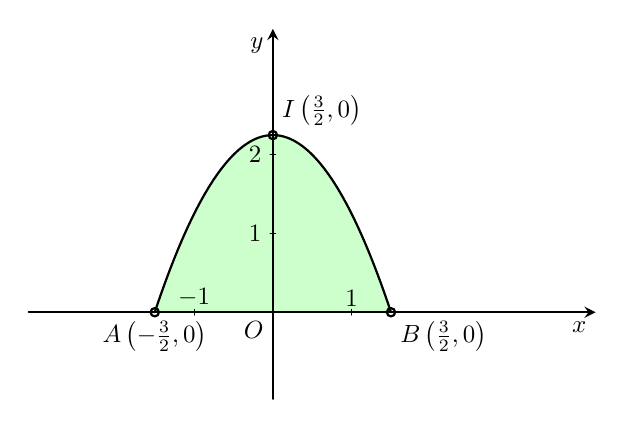
\begin{tikzpicture}[line join=round, line cap=round,>=stealth,thick]
				\tikzset{every node/.style={scale=0.9}}
				\begin{scope}
					\clip (-3,-1) rectangle (3,3.5);
					\draw[fill=green!20](-1.5,0)--plot[samples=200,domain=-1.5:1.5,smooth,variable=\x] (\x,{-1*(\x)^2+9/4})--(1.5,0);
					\draw (-1.5,0) circle (1.5pt) node[below]{$A\left(-\frac{3}{2},0\right)$};
					\draw (1.5,0) circle (1.5pt) node[below right]{$B\left(\frac{3}{2},0\right)$};
					\draw (0,2.25) circle (1.5pt) node[above right]{$I\left(\frac{3}{2},0\right)$};
				\end{scope}
				\draw[->] (-3.1,0)--(4.1,0) node[below left] {$x$};
				\draw[->] (0,-1.1)--(0,3.6) node[below left] {$y$};
				\draw (0,0) node [below left] {$O$};
				\foreach \x/\nx in {-1/-1,1/1}
				\draw[thin] (\x,1pt)--(\x,-1pt) node [above] {$\nx$};
				\foreach \y/\ny in {1/1,2/2}
				\draw[thin] (1pt,\y)--(-1pt,\y) node [left] {$\ny$};
			\end{tikzpicture}
		}
		\noindent
		Dựa vào đồ thị, diện tích của parabol là
		\[S=\displaystyle\int\limits_{-\tfrac{3}{2}}^{\tfrac{3}{2}}{\left(-x^2+\dfrac{9}{4}\right)\mathrm{\,d}x}=2\displaystyle\int\limits_0^{\tfrac{3}{2}}{\left(-x^2+\dfrac{9}{4}\right)\mathrm{\,d}x}=2\left(\dfrac{-x^3}{3}+\dfrac{9}{4}x\right)\Bigg|_0^{\tfrac{9}{4}}=\dfrac{9}{2}\,\mathrm{(m^2)}.\]
		Số tiền phải trả là $\dfrac{9}{2}\cdot 1\,500\,000=6\,750\,000$\,(đồng).
	}
\end{ex}

%Câu 2
\begin{ex}%[2D4V3-2]
	\immini{Chị Minh Hiền muốn làm một cái cổng hình Parabol như hình vẽ bên. Chiều cao $GH=4$\,m, chiều rộng $AB=4$\,m, $AC=BD=0{,}9$\,m. Chị Minh Hiền làm hai cánh cổng khi đóng lại là hình chữ nhật $CDEF$ tô đậm có giá là $1\,200\,000$\,đồng/$\mathrm{m^2}$, còn các phần để trắng làm xiên hoa có giá là $900\,000$\,đồng/$\mathrm{m^2}$. Hỏi tổng số tiền để làm hai phần nói trên gần nhất với số tiền nào dưới đây?
		\choice
		{\True $11\,445\,000$\,đồng}
		{$4\,077\,000$\,đồng}
		{$7\,368\,000$\,đồng}
		{$11\,370\,000$\,đồng}
	}{
		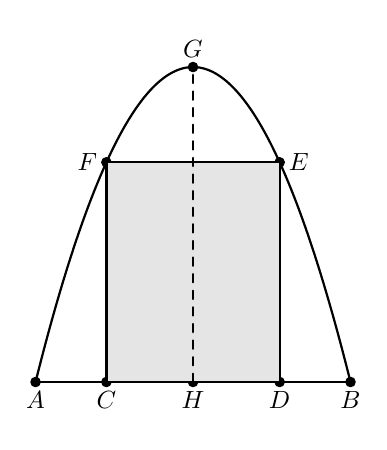
\begin{tikzpicture}[line join=round, line cap=round,>=stealth,thick]
			\tikzset{every node/.style={scale=0.9}}
			\begin{scope}
				\clip (-0.1,-0.5) rectangle (4.1,4.5);
				\draw(0,0)--plot[samples=200,domain=0:4,smooth,variable=\x] (\x,{-1*(\x)^2+4*(\x)})--(4,0);
				\draw[fill=black](0,0) circle (1.5pt) node[below]{$A$} (4,0) circle (1.5pt) node[below]{$B$} (2,4) circle (1.5pt) node[above]{$G$} (0.9,2.79) circle (1.5pt) node[left]{$F$} (3.1,2.79) circle (1.5pt) node[right]{$E$} (3.1,0) circle (1.5pt) node[below]{$D$} (0.9,0) circle (1.5pt) node[below]{$C$} (2,0) circle (1.5pt) node[below]{$H$};
				\draw[fill=gray!20](0.9,0)--(0.9,2.79)--(3.1,2.79)--(3.1,0) (0,0)--(4,0);
				\draw[dashed](2,0)--(2,4);
			\end{scope}
		\end{tikzpicture}
	}
	\loigiai{
		\immini{Gắn hệ trục tọa độ Oxy sao cho $AB$ trùng $Ox$, $A$ trùng $O$ khi đó parabol có đỉnh $G(2;4)$ và đi qua gốc tọa độ.\\
			Giả sử phương trình của parabol có dạng $y=ax^2+bx+c$, $(a\ne 0)$.\\
			Vì parabol có đỉnh là $G(2;4)$ và đi qua điểm $O(0;0)$ nên ta có \[\heva{&c=0\\&-\dfrac{b}{2a}=2\\&a\cdot 2^2+b\cdot 2+c=4}\Leftrightarrow\heva{&a=-1\\&b=4\\&c=0.}\]
		}{
			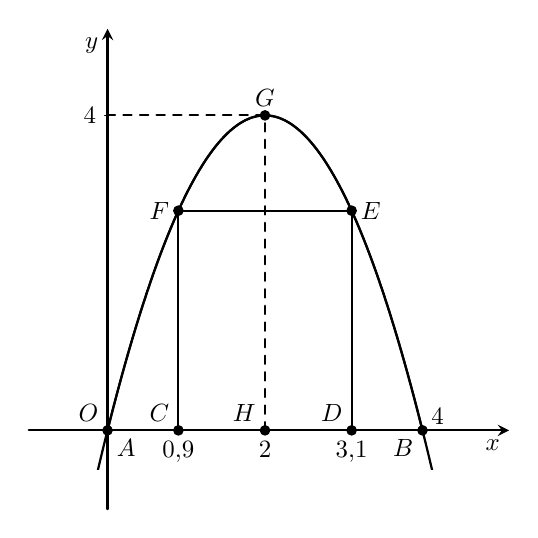
\begin{tikzpicture}[line join=round, line cap=round,>=stealth,thick]
				\tikzset{every node/.style={scale=0.9}}
				\begin{scope}
					\clip (-0.5,-0.5) rectangle (4.5,4.5);
					\draw(0,0)--plot[samples=200,domain=0:4,smooth,variable=\x] (\x,{-1*(\x)^2+4*(\x)})--(4,0);
					\draw plot[samples=200,domain=-0.5:4.5,smooth,variable=\x] (\x,{-1*(\x)^2+4*(\x)});
					\draw[fill=black](0,0) circle (1.5pt) node[below right]{$A$} (4,0) circle (1.5pt) node[below left]{$B$} (2,4) circle (1.5pt) node[above]{$G$} (0.9,2.79) circle (1.5pt) node[left]{$F$} (3.1,2.79) circle (1.5pt) node[right]{$E$} (3.1,0) circle (1.5pt) node[above left]{$D$} (0.9,0) circle (1.5pt) node[above left]{$C$} (2,0) circle (1.5pt) node[above left]{$H$};
					\draw(0.9,0)--(0.9,2.79)--(3.1,2.79)--(3.1,0) (0,0)--(4,0);
					\draw[dashed](2,0)--(2,4)--(0,4);
				\end{scope}
				\draw[->] (-1,0)--(5.1,0) node[below left] {$x$};
				\draw[->] (0,-1)--(0,5.1) node[below left] {$y$};
				\draw (0,0) node [above left] {$O$};
				\foreach \x/\nx in {0.9/0{,}9,2/2,3.1/3{,}1}
				\draw[thin] (\x,1pt)--(\x,-1pt) node [below] {$\nx$};
				\draw[thin] (4,1pt)--(4,-1pt) node [above right] {$4$};
				\foreach \y/\ny in {4/4}
				\draw[thin] (1pt,\y)--(-1pt,\y) node [left] {$\ny$};
			\end{tikzpicture}				
		}
		\noindent
		Suy ra phương trình parabol là $y=f(x)=-x^2+4x$.\\
		Diện tích của cả cổng là $S=\displaystyle\int\limits_0^4\left(-x^2+4x\right)\mathrm{\,d}x=\left(-\dfrac{x^3}{3}+2x^2\right)\Bigg|_0^4=\dfrac{32}{3}\,\mathrm{\left(m^2\right)}$.\\
		Mặt khác chiều cao $CF=DE=f(0{,}9)=2{,}79$\,(m); $CD=4-2\cdot 0{,}9=2{,}2$\,(m).\\
		Diện tích hai cánh cổng là $S_{CDEF}=CD\cdot CF=6{,}138\,\mathrm{(m^2)}$.\\
		Diện tích phần xiên hoa là $S_{xh}=S-S_{CDEF}=\dfrac{32}{3}-6{,}14=\dfrac{6793}{1500}\,\mathrm{(m^2)}$.\\
		Vậy tổng số tiền để làm cổng là $6{,}138\cdot 1\,200\,000+\dfrac{6793}{1500}\cdot 900\,000=11\,441\,400$\,(đồng).
	}
\end{ex}

%Câu 3
\begin{ex}%[2D4V3-2]
	\immini{Một cổng chào có dạng hình Parabol chiều cao $18$\,m, chiều rộng chân đế $12$\,m. Người ta căng hai sợi dây trang trí $AB$, $CD$ nằm ngang đồng thời chia hình giới hạn bởi Parabol và mặt đất thành ba phần có diện tích bằng nhau (xem hình vẽ bên). Tỉ số $\dfrac{AB}{CD}$ bằng
		\choice
		{$\dfrac{1}{\sqrt{2}}$}
		{$\dfrac{4}{5}$}
		{\True $\dfrac{1}{\sqrt[3]{2}}$}
		{$\dfrac{3}{1+2\sqrt{2}}$}
	}{
		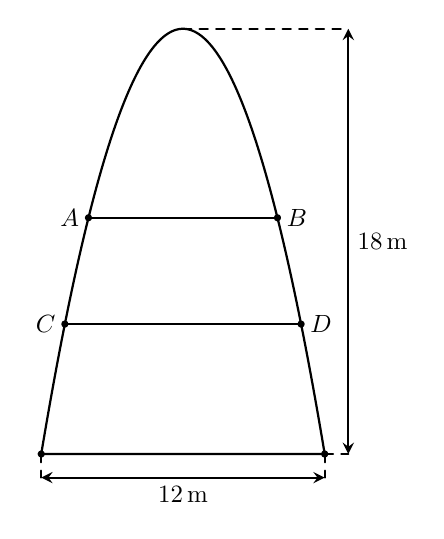
\begin{tikzpicture}[line join=round, line cap=round,>=stealth,thick,scale=0.6]
			\tikzset{every node/.style={scale=0.9}}
			\begin{scope}
				\draw(-3,-9)--plot[samples=200,domain=-3:3,smooth,variable=\x] (\x,{-1*(\x)^2})--(3,-9)--cycle;
				\draw[dashed](0,0)--(3.5,0) (3,-9)--(3.5,-9) (-3,-9)--(-3,-9.5) (3,-9)--(3,-9.5);
				\draw[<->](3.5,0)--(3.5,-9) node[pos=0.5, right]{$18$\,m}; \draw[<->](-3,-9.5)--(3,-9.5) node[pos=0.5, below]{$12$\,m};
				\draw[fill=black](-2,-4) circle (1.5pt) node[left]{$A$} (2,-4) circle (1.5pt) node[right]{$B$} (-2.5,-6.25) circle (1.5pt) node[left]{$C$} (2.5,-6.25) circle (1.5pt) node[right]{$D$} (-3,-9) circle (1.5pt) (3,-9) circle (1.5pt);
				\draw (-2,-4)--(2,-4) (-2.5,-6.25)--(2.5,-6.25);
			\end{scope}
		\end{tikzpicture}
	}
	\loigiai{
		\immini{Chọn hệ trục tọa độ $Oxy$ như hình vẽ.
			Phương trình Parabol $(P)$ có dạng $y=ax^2$.\\
			$(P)$ đi qua điểm có tọa độ $(-6;-18)$.\\
			Suy ra $-18=a\cdot (-6)^2\Leftrightarrow a=-\dfrac{1}{2}.\\
			\Rightarrow(P)\colon y=-\dfrac{1}{2}x^2$.\\
			Từ hình vẽ ta có $\dfrac{AB}{CD}=\dfrac{x_1}{x_2}$.\\
			Diện tích hình phẳng giới bạn bởi Parabol và đường thẳng $AB\colon y=-\dfrac{1}{2}x_1^2$ là
			\allowdisplaybreaks
			\begin{eqnarray*}
				S_1&=&2\displaystyle\int\limits_0^{x_1}{\left[-\dfrac{1}{2}{x^2}-\left(-\dfrac{1}{2}x_1^2\right)\right]\mathrm{\,d}x}\\
				&=&2\left(-\dfrac{1}{2}\cdot \dfrac{x^3}{3}+\dfrac{1}{2}x_1^2x\right)\Bigg|_0^{x_1}=\dfrac{2}{3}x_1^3.
			\end{eqnarray*}
		}{
			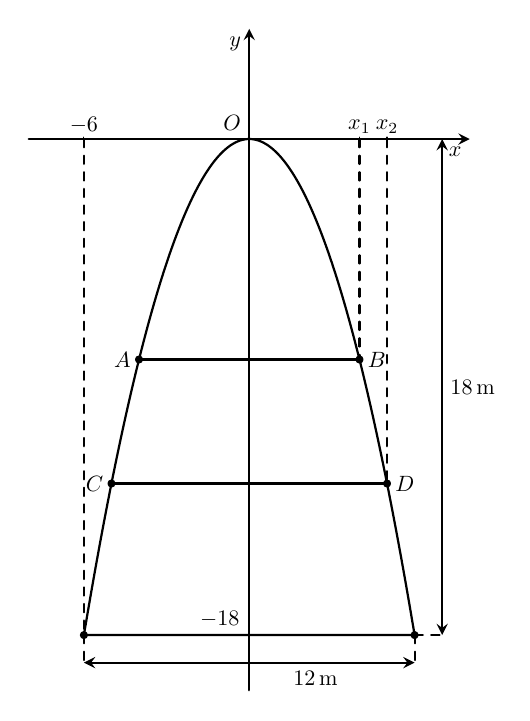
\begin{tikzpicture}[line join=round, line cap=round,>=stealth,thick,scale=0.7]
				\tikzset{every node/.style={scale=0.8}}
				\begin{scope}
					\draw(-3,-9)--plot[samples=200,domain=-3:3,smooth,variable=\x] (\x,{-1*(\x)^2})--(3,-9)--cycle;
					\draw[dashed] (3,-9)--(3.5,-9) (-3,-9)--(-3,-9.5) (3,-9)--(3,-9.5);
					\draw[<->](3.5,0)--(3.5,-9) node[pos=0.5, right]{$18$\,m}; \draw[<->](-3,-9.5)--(3,-9.5) node[pos=0.7, below]{$12$\,m};
					\draw[fill=black](-2,-4) circle (1.5pt) node[left]{$A$} (2,-4) circle (1.5pt) node[right]{$B$} (-2.5,-6.25) circle (1.5pt) node[left]{$C$} (2.5,-6.25) circle (1.5pt) node[right]{$D$} (-3,-9) circle (1.5pt) (3,-9) circle (1.5pt);
					\draw (-2,-4)--(2,-4) (-2.5,-6.25)--(2.5,-6.25);
				\end{scope}
				\draw[->] (-4,0)--(4,0) node[below left] {$x$};
				\draw[->] (0,-10)--(0,2.0) node[below left] {$y$};
				\draw (0,0) node [above left] {$O$};
				\foreach \x/\nx in {-3/-6,2/x_1,2.5/x_2}
				\draw[thin] (\x,1pt)--(\x,-1pt) node [above] {$\nx$};
				\draw[thin] (1pt,-9)--(-1pt,-9) node [above left] {$-18$};
				\draw[dashed](-3,0)--(-3,-9) (2,0)--(2,-4) (2.5,0)--(2.5,-6.25);
			\end{tikzpicture}
		}
		\noindent
		Diện tích hình phẳng giới hạn bởi Parabol và đường thẳng $CD\colon y=-\dfrac{1}{2}x_2^2$ là
		\[S_2=2\displaystyle\int\limits_0^{x_2}{\left[-\dfrac{1}{2}{x^2}-\left(-\dfrac{1}{2}x_2^2\right)\right]\mathrm{\,d}x}=2\left(-\dfrac{1}{2}\cdot \dfrac{x^3}{3}+\dfrac{1}{2}x_2^2x\right)\Bigg|_0^{x_2}=\dfrac{2}{3}x_2^3.\]
		Từ giả thiết suy ra $S_2=2S_1\Leftrightarrow x_2^3=2x_1^3\Leftrightarrow\dfrac{x_1}{x_2}=\dfrac{1}{\sqrt[3]{2}}$.\\
		Vậy $\dfrac{AB}{CD}=\dfrac{x_1}{x_2}=\dfrac{1}{\sqrt[3]{2}}$.
	}
\end{ex}

%Câu 4
\begin{ex}%[2D4C3-2]
	\immini{Một họa tiết hình cánh bướm như hình vẽ bên. Phần tô đậm được đính đá với giá thành $500\,000$/$\,\mathrm{m^2}$. Phần còn lại được tô màu với giá thành $250\,000$/$\,\mathrm{m^2}$. Cho $AB=4$\,dm; $BC=8$\,dm. Hỏi để trang trí $1\,000$ họa tiết như vậy cần số tiền gần nhất với số nào sau đây.
		\choice
		{$105\,660\,667$}
		{\True $106\,666\,667$}
		{$ 107\,665\,667$}
		{$ 108\,665\,667$}
	}{
		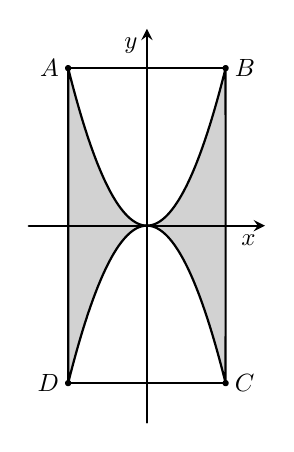
\begin{tikzpicture}[line join=round, line cap=round,>=stealth,thick,scale=0.5]
			\tikzset{every node/.style={scale=0.9}}
			\begin{scope}
				\draw[fill=gray!35](-2,0)--plot[samples=200,domain=-2:2,smooth,variable=\x] (\x,{(\x)^2})--(2,0);
				\draw[fill=gray!35](-2,0)--plot[samples=200,domain=-2:2,smooth,variable=\x] (\x,{-1*(\x)^2})--(2,0);
				\draw[fill=black](-2,4) circle (1.5pt) node[left]{$A$} (2,4) circle (1.5pt) node[right]{$B$} (2,-4) circle (1.5pt) node[right]{$C$} (-2,-4) circle (1.5pt) node[left]{$D$};
				\draw (-2,4)--(2,4) (2,-4)--(-2,-4);
			\end{scope}
			\draw[->] (-3,0)--(3,0) node[below left] {$x$};
			\draw[->] (0,-5)--(0,5) node[below left] {$y$};
		\end{tikzpicture}
	}
	\loigiai{
		Vì $AB=4$\,dm; $BC=8$\,dm $\Rightarrow A(-2;4)$, $B(2;4)$, $C(2;-4)$, $D(-2;-4)$.\\
		parabol là $y=x^2$ hoặc $y=-x^2$.\\
		Diện tích phần tô đậm là $S_1=4\displaystyle\int\limits_0^2{x^2}\mathrm{\,d}x=\dfrac{32}{3}\mathrm{\,(dm^2)}$.\\
		Diện tích hình chữ nhật là $S=4\cdot 8=32\mathrm{\,(dm^2)}$.\\
		Diện tích phần trắng là $S_2=S-S_1=32-\dfrac{32}{3}=\dfrac{64}{3}\mathrm{\,(dm^2)}$.\\
		Tổng chi phí trang chí là $T=\left(\dfrac{32}{3}\cdot 5\,000+\dfrac{64}{3}\cdot 2\,500\right)\cdot 1\,000\approx 106\,666\,667$.
	}
\end{ex}
%%==========Câu 5
% \begin{ex}%[2D4C3-2]
% 	\immini{Một hoa văn trang trí được tạo ra từ một miếng bìa mỏng hình vuông cạnh bằng $10$ cm bằng cách khoét đi bốn phần bằng nhau có hình dạng parabol như hình bên. Biết $AB=5$ cm, $OH=4$ cm. Biết giá trang trí hoa văn $1$ cm$^2$ là $50000$ đồng, tính số tiền cần bỏ ra để trang trí hoa văn đó.
% 		\choice
% 		{$2\,553\,333$ đồng}
% 		{\True $2\,333\,333$ đồng}
% 		{$2\,780\,333$ đồng}
% 		{$2\,123\,333$ đồng}
% 	}{
% 		\begin{tikzpicture}[line join=round, line cap=round,>=stealth,thick,scale=0.5]
% 			\tikzset{every node/.style={scale=0.9}}
% 			\begin{scope}
% 				\fill[black] (0,0)--(10,0)--(10,10)--(0,10)--cycle;
% 				\fill[white](2.5,0)--plot[samples=200,domain=2.5:7.5,smooth,variable=\x] (\x,{-16/25*(\x-2.5)^2+16/5*(\x-2.5)})--(7.5,0);
% 				\fill[white](2.5,10)--plot[samples=200,domain=2.5:7.5,smooth,variable=\x] (\x,{16/25*(\x-2.5)^2-16/5*(\x-2.5)+10})--(7.5,10);
% 				\fill[white] plot[samples=200,domain=6:10,smooth,variable=\x] (\x,{sqrt(1.5625*((\x)-6))+5})--(10,5)--plot[samples=200,domain=6:10,smooth,variable=\x] (\x,{-sqrt(1.5625*((\x)-6))+5})--(10,5);
% 				\fill[white] plot[samples=200,domain=4:0,smooth,variable=\x] (\x,{sqrt(1.5625*(4-(\x)))+5})--(0,5)--plot[samples=200,domain=4:0,smooth,variable=\x] (\x,{-sqrt(1.5625*(4-(\x)))+5})--(0,5);				
% 			\end{scope}
% 			\draw[fill=white](6,5) circle (1.5pt) node[above right]{$O$} (10,2.5) circle (1.5pt) node[right]{$B$} (10,7.5) circle (1.5pt) node[right]{$A$} (10,5) circle (1.5pt) node[right]{$H$};
% 			\draw[dashed] (6,5)--(10,5) (10,2.5)--(10,7.5);
% 		\end{tikzpicture}
% 	}
% 	\loigiai{
% 		\immini{Đưa parabol vào hệ trục $Oxy$ ta tìm được phương trình là $(P)\colon y=-\dfrac{16}{25}x^2+\dfrac{16}{5}x$.\\
% 			Diện tích hình phẳng giới hạn bởi $(P)\colon y=-\dfrac{16}{25}x^2+\dfrac{16}{5}x$, trục hoành và các đường thẳng $x=0$, $x=5$ là
% 			\[S=\displaystyle\int\limits_0^5 \left(-\dfrac{16}{25}x^2+\dfrac{16}{5}x\right)\mathrm{\,d}x=\dfrac{40}{3}.\]
			
% 		}
% 		{\begin{tikzpicture}[line join=round, line cap=round,>=stealth,thick,scale=0.7]
% 				\tikzset{every node/.style={scale=0.8}}
% 				\draw[step=0.5, gray!50,very thin] (0,0) grid (5.5,4.5);
% 				\draw[->] (-0.5,0)--(6.1,0) node[below left] {$x$};
% 				\draw[->] (0,-0.5)--(0,5.1) node[below left] {$y$};
% 				\foreach \x/\nx in {1/1,2/2,3/3,4/4,5/5}
% 				\draw[thin] (\x,1pt)--(\x,-1pt) node [below] {$\nx$};
% 				\foreach \y/\ny in {1/1,2/2,3/3,4/4}
% 				\draw[thin] (1pt,\y)--(-1pt,\y) node [left] {$\ny$};
% 				\draw (0,0) node [below left] {$O$};
% 				\begin{scope}
% 					\clip (-0.5,-0.5) rectangle (5.5,5);
% 					\draw[samples=200,domain=-0.5:5.5,smooth,variable=\x] plot (\x,{-0.64*(\x)^2+3.2*(\x)+0});
% 				\end{scope}
% 				\draw[fill=black](0,0) circle (1.5pt) (2.5,4) circle (1.5pt) (5,0) circle (1.5pt);
% 			\end{tikzpicture}
% 		}\noindent
% 		Tổng diện tích phần bị khoét đi $S_1=4S=\dfrac{160}{3}$ cm$^2$.\\
% 		Diện tích của hình vuông là $S_{hv}=100$ cm$^2$.\\
% 		diện tích bề mặt hoa văn là $S_2=S_{hv}-S_1=100-\dfrac{160}{3}=\dfrac{140}{3}\mathrm{\,(cm^2)}$.\\
% 		Vậy số tiền cần bỏ ra để trang trí hoa văn đó là $\dfrac{140}{3}\cdot 50\,000\approx 2\,333\,333$ (đồng).
% 	}
% \end{ex}
%%==========Câu 6
\begin{ex}%[2D4V3-2]
	\immini{Một viên gạch hoa hình vuông cạnh $40$ cm. Người thiết kế đã sử dụng bốn đường parabol có chung đỉnh tại tâm viên gạch để tạo ra bốn cánh hoa (được tô đen như hình vẽ dưới). Diện tích mỗi cánh hoa của viên gạch bằng
		\choice
		{$800$ cm$^2$} 
		{$\dfrac{800}{3}$ cm$^2$} 
		{\True $\dfrac{400}{3}$ cm$^2$} 
		{$250$ cm$^2$}
	}
	{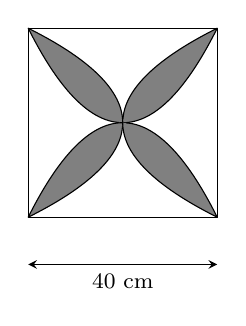
\begin{tikzpicture}[scale=1.2,>=stealth, line join = round, line cap = round,font=\footnotesize]
			\draw (-1,1) rectangle (1,-1);
			\foreach \i in {0,90,180,270}
			\draw [fill=gray, smooth, samples=100,rotate=\i] plot [domain=0:1] (\x, {(\x)^2})-- plot [domain=1:0] (\x, {sqrt(\x)});
			\draw [<-] (-1,-1.5)--(0,-1.5) node[below] {$40$ cm};
			\draw [->] (0,-1.5)--(1,-1.5);
		\end{tikzpicture}
	} 
	\loigiai{
		\immini{Chọn hệ tọa độ như hình vẽ (1 đơn vị trên trục bằng $10$ cm= $1$ dm), các cánh hoa tạo bởi các đường parabol có phương trình $ y=\dfrac{x^2}{2}$, $y=-\dfrac{x^2}{2}$, $x=-\dfrac{y^2}{2}$, $x=\dfrac{y^2}{2}$.\\ 
			Diện tích một cánh hoa (nằm trong góc phàn tư thứ nhất) bằng diện tích hình phẳng giới hạn bởi hai đồ thị hàm số $y=\dfrac{x^2}{2}$, $y=\sqrt{2x}$ và hai đường thẳng $ x=0$; $x=2$.
		}
		{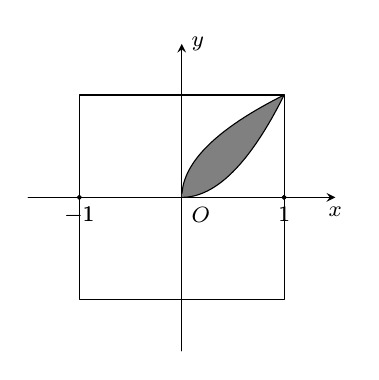
\begin{tikzpicture}[scale=1.3,>=stealth, line join = round, line cap = round,font=\footnotesize]
				\draw[->] (-1.5,0)--(0,0)%
				node[below right]{$O$}--(1.5,0) node[below]{$x$};
				\draw[->] (0,-1.5) --(0,1.5) node[right]{$y$};
				\draw (-1,1) rectangle (1,-1);
				\foreach \i in {-1,1}
				\foreach \j in {-1,1}
				\draw[fill=black]  (\i,0) circle (0.5 pt) node [below] {\footnotesize $\i$};
				\draw [fill=gray, smooth, samples=100] plot [domain=0:1] (\x, {(\x)^2})-- plot [domain=1:0] (\x, {sqrt(\x)});
			\end{tikzpicture}
		}\noindent
		Do đó diện tích một cánh hoa bằng 
		\[\displaystyle\int\limits_0^2 \left( \sqrt{2x}-\dfrac{x^2}{2} \right) \mathrm{d}x = \left(\dfrac{2\sqrt{2}}{3}\sqrt{(2x)^3}-\dfrac{x^3}{6} \right) \Big|_0^2 = \dfrac{4}{3} \;\;\text{dm}^2= \dfrac{400}{3}\;\;\text{cm}^2.\]
	}
\end{ex} 
\Closesolutionfile{ans}
\indapan{6}{ans/ans-2-C4B3CD3_1-4-lc}

% \begin{dang}
% 	{Ứng dụng thể tích khối tròn xoay trong bài toán thực tiễn}
% \end{dang}
\Opensolutionfile{ans}[ans/ans-2-C4B3CD3_1-2-lc]
%%==========Câu 7
% \begin{ex}%[2D4V3-4]
% 	\immini{Khi cắt một vật thể hình chiếc niêm bởi mặt phẳng vuông góc với trục $Ox$ tại điểm có hoành độ $x$ ($-2 \le x\le 2$), mặt cắt là tam giác vuông có một góc $45^\circ$ và độ dài một cạnh góc vuông là $\sqrt{14-3x^2}$ (như hình vẽ). Tính thể tích vật thể hình chiếc niêm trên.
% 		\choice
% 		{\True $V=20$}
% 		{$V=20\pi$}
% 		{$V=10$}
% 		{$V=10\pi$}
% 	}
% 	{\begin{tikzpicture}[declare function={r=4;d=3;},scale=0.6]
% 			\path (0,0) coordinate (O)--++(85:r/3) coordinate (A)
% 			($(A)!2!(O)$) coordinate (B)
% 			($(O)+(0:r)$) coordinate (C)
% 			($(C)+(90:d)$) coordinate (D)
% 			;
% 			\draw (A)..controls +(40:1.5) and +(90:1)..(D)..controls +(-90:1) and +(40:1.5)..(B);
% 			\draw (A)--(O)node[midway,left]{} (O)--(B)node[midway,left]{} (C)--(D)
% 			(C)..controls +(-90:1) and +(0:2)..(B)
% 			;
% 			\draw[dashed] 
% 			(A)..controls +(0:2) and +(90:1)..(C)
% 			(D)--(O) (O)--(C)node[pos=0.7,above]{} ;
% 			\path pic[draw,angle radius=17pt,"$\alpha$"]{angle= C--O--D};
% 		\end{tikzpicture}
% 	}
% 	\loigiai{
% 		Diện tích tam giác vuông cân là $S(x)=\dfrac{1}{2}\sqrt{14-3x^2} \cdot \sqrt{14-3x^2} = \dfrac{1}{2}(14-3x^2)$.\\
% 		Vậy thể tích vật thể là $\displaystyle\int\limits_{-2}^2 \dfrac{1}{2}(14-3x^2)\mathrm{\,d}x=20$.
% 	}
% \end{ex}
%%==========Câu 8
% \begin{ex}%[2D4V3-4]
% 	\immini{Trong chương trình nông thôn mới của tỉnh Phú Yên, tại xã Hòa Mỹ Tây có xây một cây cầu bằng bê tông như hình vẽ (đường cong trong hình vẽ là các đường Parabol). Biết $1$ m$^3$ khối bê tông để đổ cây cầu có giá 5 triệu đồng. Tính số tiền mà tỉnh Phú Yên cần bỏ ra để xây cây cầu trên.
% 	}
% 	{\begin{tikzpicture}[scale=1.0, font=\footnotesize, line join=round, line cap=round,>=stealth,samples=100]
% 			\path 
% 			(0,0) coordinate (O)
% 			(-1,0) coordinate (B)
% 			(0,1) coordinate (C)
% 			(1,0) coordinate (D)
% 			(-1.4,0) coordinate (M)
% 			(0,1.96) coordinate (N)
% 			(1.4,0) coordinate (P)
% 			;
% 			\path (-165:4) coordinate (A);
% 			\foreach \x in {B,C,D,M,N,P,O}{\path ($(\x)+(-165:4)$) coordinate (\x_1);}
% 			\fill[gray!40] (N_1)--(N)--plot[domain=0:1.4] (\x,{-(\x)^2+1.96})--(P)--(P_1)--plot[shift={(A)},domain=1.4:0] (\x,{-(\x)^2+1.96});
% 			\fill[gray!40] (M_1)--plot[shift={(A)},domain=-1.4:1.4](\x,{-(\x)^2+1.96})--(P_1)--(D_1)--plot[shift={(A)},domain=1:-1] (\x,{-(\x)^2+1})--(B_1)--(M_1);
% 			\draw[dash pattern=on 2pt off 2pt] plot[domain=-1:1] (\x,{-(\x)^2+1})
% 			plot[domain=-1.4:1.4] (\x,{-(\x)^2+1.96})
% 			(M)--(P) (O)--(N)
% 			;
% 			\draw[shift={(A)}] plot[domain=-1:1] (\x,{-(\x)^2+1});
% 			\draw[shift={(A)}] plot[domain=-1.4:1.4] (\x,{-(\x)^2+1.96});
% 			\draw [dash pattern=on 2pt off 2pt] (B)--(B_1) (C)--(C_1) (D)--(D_1) (M)--(M_1)
% 			(O_1)--(N_1)
% 			;
% 			\draw (N)--(N_1) (P)--(P_1) (M_1)--(P_1);
% 			\foreach \t in {O,B,M,P,O_1,M_1,B_1,D_1,P_1}{
% 				\draw[fill=white] (\t) circle (1pt);}
% 			\path (M_1)--(B_1) node[midway,below]{$0,5$m};
% 			\path (B_1)--(D_1) node[midway,below]{$19$m};
% 			\path (D_1)--(P_1) node[midway,below]{$0,5$m};
% 			\path (O)--(C) node[midway,right]{$2$m};
% 			\path (C)--(N) node[pos=0.2,left]{$0,5$m};
% 		\end{tikzpicture}
% 	}
% 	\choice
% 	{$110$ triệu đồng}
% 	{$250$ triệu đồng}
% 	{$180$ triệu đồng}
% 	{\True $200$ triệu đồng}
% 	\loigiai{
% 		\immini{Chọn hệ trục $Oxy$ như hình vẽ.\\
% 			Gọi $(P_1)\colon y=a_1 x^2+b_1$ là Parabol đi qua hai điểm $A\left(\dfrac{19}{2};0\right)$, $B(0;2)$.\\
% 		}
% 		{\begin{tikzpicture}[scale=0.9, font=\footnotesize, line join=round, line cap=round,>=stealth,samples=100]
% 				\path 
% 				(0,0) coordinate (O)
% 				(-1,0) coordinate (B)
% 				(0,1) coordinate (C)
% 				(1,0) coordinate (D)
% 				(-1.4,0) coordinate (M)
% 				(0,1.96) coordinate (N)
% 				(1.4,0) coordinate (P)
% 				;
% 				\path (-165:4) coordinate (A);
% 				\foreach \x in {B,C,D,M,N,P,O}{\path ($(\x)+(-165:4)$) coordinate (\x_1);}
% 				\fill[gray!40] (N_1)--(N)--plot[domain=0:1.4] (\x,{-(\x)^2+1.96})--(P)--(P_1)--plot[shift={(A)},domain=1.4:0] (\x,{-(\x)^2+1.96});
% 				\fill[gray!40] (M_1)--plot[shift={(A)},domain=-1.4:1.4](\x,{-(\x)^2+1.96})--(P_1)--(D_1)--plot[shift={(A)},domain=1:-1] (\x,{-(\x)^2+1})--(B_1)--(M_1);
% 				\draw[-stealth,dash pattern=on 2pt off 2pt] (-1.4,0)--(0,0)node[below left]{$O$}--(2,0) node[below] {$x$};
% 				\draw[-stealth,dash pattern=on 2pt off 2pt] (0,0)--(0,2.5) node[left] {$y$};
% 				\draw[dash pattern=on 2pt off 2pt] plot[domain=-1:1] (\x,{-(\x)^2+1})
% 				plot[domain=-1.4:1.4] (\x,{-(\x)^2+1.96})
% 				;
% 				\draw[shift={(A)}] plot[domain=-1:1] (\x,{-(\x)^2+1});
% 				\draw[shift={(A)}] plot[domain=-1.4:1.4] (\x,{-(\x)^2+1.96});
% 				\draw [dash pattern=on 2pt off 2pt] (B)--(B_1) (C)--(C_1) (D)--(D_1) (M)--(M_1)
% 				(O_1)--(N_1)
% 				;
% 				\draw (N)--(N_1) (P)--(P_1) (M_1)--(P_1);
% 				\foreach \t in {O,B,M,P,O_1,M_1,B_1,D_1,P_1}{
% 					\draw[fill=white] (\t) circle (1pt);}
% 				\path (M_1)--(B_1) node[midway,below]{$0,5$m};
% 				\path (B_1)--(D_1) node[midway,below]{$19$m};
% 				\path (D_1)--(P_1) node[midway,below]{$0,5$m};
% 				\path (O)--(C) node[midway,right]{$2$m};
% 				\path (C)--(N) node[pos=0.2,left]{$0,5$m};
% 			\end{tikzpicture}
% 		}\noindent
% 		Nên ta có hệ phương trình sau
% 		\[\heva{& 0=a\cdot \left(\dfrac{19}{2}\right)^2+2 \\ & 2=b} \Leftrightarrow \heva{& a_1=-\dfrac{8}{361} \\ & b_1=2 }\Rightarrow (P_1)\colon y=-\dfrac{8}{361}{x^2}+2.\]
% 		Gọi $(P_2)\colon y=a_2 x^2+b_2$ là Parabol đi qua hai điểm $C(10;0)$, $D\left(0;\dfrac{5}{2}\right)$.\\
% 		Nên ta có hệ phương trình sau
% 		\[\heva{& 0=a_2 \cdot 10^2 + \dfrac{5}{2} \\ & \dfrac{5}{2}=b_2 } \Leftrightarrow \heva{& a_2=-\dfrac{1}{40} \\ & b_2=\dfrac{5}{2} } \Rightarrow (P_2)\colon y=-\dfrac{1}{40}{x^2}+\dfrac{5}{2}.\]
% 		Ta có thể tích của bê tông là
% 		\[V=5\cdot 2\left[\displaystyle\int\limits_0^{10}\left(-\dfrac{1}{40}{x^2}+\dfrac{5}{2} \right)\mathrm{\,d}x-\displaystyle\int\limits_0^{\tfrac{19}{2}}\left( -\dfrac{8}{361}x^2+2\right)\mathrm{\,d}x \right]=40\;\;\text{m}^3.\]
% 		Số tiền mà tỉnh Phú Yên cần bỏ ra để xây cây cầu là $5\cdot 40=200$ triệu đồng.
% 	}
% \end{ex}
%%==========Câu 9
\begin{ex}%[2D4V3-4]
	Để kỷ niệm ngày 26-3. Chi đoàn 12A dự định dựng một lều trại có dạng parabol, với kích thước: nền trại là một hình chữ nhật có chiều rộng là $3$ mét, chiều sâu là $6$ mét, đỉnh của parabol cách mặt đất là $3$ mét. Hãy tính thể tích phần không gian phía bên trong trại để lớp 12A cử số lượng người tham dự trại cho phù hợp.
	\choice
	{$30$ m$^3$}
	{\True $36$ m$^3$}
	{$40$ m$^3$}
	{$41$ m$^3$}
	\loigiai{
		Giả sử nền trại là hình chữ nhật $ABCD$ có $AB = 3$ m, $BC = 6$ m, đỉnh của parabol là $I$.\\
		Chọn hệ trục tọa độ $Oxy$ sao cho $O$ là trung điểm của cạnh $AB$, $A$, $B$ và $I$, phương trình của parabol có dạng $y=ax^2+b$, $a \ne 0$.\\
		Do $I$, $A$, $B$ thuộc nên ta có $y=-\dfrac{4}{3}x^2+3$.\\
		Vậy thể tích phần không gian phía trong trại là
		\[V=6 \cdot 2\displaystyle\int\limits_0^{\tfrac{3}{2}}\left(-\dfrac{4}{3}x^2+3\right)\mathrm{\,d}x=36.\]
	}
\end{ex}
%%==========Câu 10
\begin{ex}%[2D4V3-4]
	Cho một vật thể bằng gỗ có dạng hình trụ với chiều cao và bán kính đáy cùng bằng $R$. Cắt khối gỗ đó bởi một mặt phẳng đi qua đường kính của một mặt đáy của khối gỗ và tạo với mặt phẳng đáy của khối gỗ một góc $30^\circ$ ta thu được hai khối gỗ có thể tích là $V_1$ và $V_2$, với $V_1<V_2$. Thể tích $V_1$ bằng
	\choice
	{\True $V_1=\dfrac{2\sqrt{3}R^3}{9}$}
	{$V_1=\dfrac{\sqrt{3}\pi R^3}{27}$}
	{$V_1=\dfrac{\sqrt{3}\pi R^3}{18}$}
	{$V_1=\dfrac{\sqrt{3}R^3}{27}$}
	\loigiai{
		\immini{Khi cắt khối gỗ hình trụ ta được một hình nêm có thể tích $V_1$ như hình vẽ.\\
			Chọn hệ trục tọa độ $Oxy$ như hình vẽ.\\
			Nửa đường tròn đường kính $AB$ có phương trình là
			\[y=\sqrt{R^2-x^2}, x \in [-R;R].\]
		}
		{\begin{tikzpicture}[declare function={r=4;d=3;},scale=0.7]
				\path (0,0) coordinate (O)--++(85:r/3) coordinate (A)
				($(A)!2!(O)$) coordinate (B)
				($(O)+(0:r)$) coordinate (C)
				($(C)+(90:d)$) coordinate (D)
				;
				\draw (A)..controls +(40:1.5) and +(90:1)..(D)..controls +(-90:1) and +(40:1.5)..(B);
				\draw (A)--(O)node[midway,left]{$R$} (O)--(B)node[midway,left]{$R$} (C)--(D)
				(C)..controls +(-90:1) and +(0:2)..(B)
				;
				\draw[dashed] 
				(A)..controls +(0:2) and +(90:1)..(C)
				(D)--(O) (O)--(C)node[pos=0.7,above]{$R$} ;
				\path pic[draw,angle radius=17pt,"$\alpha$"]{angle= C--O--D};
			\end{tikzpicture}
		}\noindent
		Một mặt phẳng vuông góc với trục $Ox$ tại điểm $M$ có hoành độ $x$, cắt hình nêm theo thiết diện là $\triangle MNP$ vuông tại $N$ và có $\widehat{PMN}=30^\circ$.\\
		Ta có $NM=y=\sqrt{R^2-x^2} \Rightarrow NP=MN \cdot \tan 30^\circ = \dfrac{\sqrt{R^2-x^2}}{\sqrt{3}}$.\\
		Do $\triangle MNP$ có diện tích $S(x)=\dfrac{1}{2}NM \cdot NP =\dfrac{1}{2}\cdot \dfrac{R^2-x^2}{\sqrt{3}}$.\\
		Thể tích hình nêm là 
		\[V_1=\displaystyle\int\limits_{-R}^R S(x)\mathrm{\,d}x=\dfrac{1}{2}\displaystyle\int\limits_{-R}^R \dfrac{R^2-x^2}{\sqrt{3}}\mathrm{\,d}x=\dfrac{1}{2\sqrt{3}}\left(R^2 x-\dfrac{1}{3}x^3 \right) \Big|_{-R}^R=\dfrac{2\sqrt{3}{R^3}}{9}.\]
		\textbf{Chú ý:} Có thể ghi nhớ công thức tính thể tích hình nêm
		$V_1=\dfrac{2}{3}{R^2}h=\dfrac{2}{3}{R^3}\tan \alpha $, trong đó $R=\dfrac{AB}{2}$, $\alpha =\widehat{PMN}$.
	}
\end{ex}
%%==========Câu 11
% \begin{ex}%[2D4V3-4]
% 	\immini{Cho một mô hình $3-D$ mô phỏng một đường hầm như hình vẽ bên. Biết rằng đường hầm mô hình có chiều dài $5$ cm; khi cắt hình này bởi mặt phẳng vuông góc với đấy của nó, ta được thiết diện là một hình parabol có độ dài đáy gấp đôi chiều cao parabol. Chiều cao của mỗi thiết diện parobol cho bởi công thức $y=3-\dfrac{2}{5}x$ cm, với $x$ cm là khoảng cách tính từ lối vào lớn hơn của đường hầm mô hình. Tính thể tích (theo đơn vị cm$^3$) không gian bên trong đường hầm mô hình (làm tròn kết quả đến hàng đơn vị).
% 		\choice
% 		{\True $29$}
% 		{$27$}
% 		{$31$}
% 		{$33$}
% 	}
% 	{\begin{tikzpicture}[scale=0.6,declare function={a=0.8;b=0.6;c=0.4;d=0.2;}]
% 			\tikzset{
% 				homothety at/.style args={#1 scaled by #2}{shift={($(#1)!#2!(0,0)$)},scale=#2},
% 			}
% 			\def\mypath{(-120:2)..controls +(90:0.6) and +(-180:0.6)..(0,3)}
% 			\def\mydot{(0,3)..controls +(0:0.25) and +(95:0.05)..(60:2)}
% 			\draw \mypath;
% 			\draw[dashed] \mydot;
% 			\path (7,0) coordinate (c1);
% 			\begin{scope}[homothety at=c1 scaled by a]
% 				\draw \mypath;
% 				\draw[dashed] \mydot;
% 			\end{scope}
% 			\begin{scope}[homothety at=c1 scaled by b]
% 				\draw \mypath;
% 				\draw[dashed] \mydot;
% 			\end{scope}
% 			\begin{scope}[homothety at=c1 scaled by c]
% 				\draw \mypath;
% 				\draw[dashed] \mydot;
% 			\end{scope}
% 			\begin{scope}[homothety at=c1 scaled by d]
% 				\draw \mypath;
% 				\draw \mydot;
% 			\end{scope}
% 			\path 
% 			(-120:2) coordinate (A)
% 			(0,3) coordinate (B)
% 			(60:2) coordinate (C)
% 			(0,0) coordinate (O);
% 			\foreach \x in {A,B,C}{\path ($(c1)!a!(\x)$) coordinate (\x_1);}
% 			\foreach \x in {A,B,C}{\path ($(c1)!b!(\x)$) coordinate (\x_2);}
% 			\foreach \x in {A,B,C}{\path ($(c1)!c!(\x)$) coordinate (\x_3);}
% 			\foreach \x in {A,B,C}{\path ($(c1)!d!(\x)$) coordinate (\x_4);}
% 			\path ($(A_4)!0.5!(B_4)$) coordinate (D);
% 			\draw (A)--(A_4) (B)--(B_4) (A_4)--(C_4)
% 			;
% 			\draw[dashed] (B)node[above]{$3$}--(O)--(D)node[below right]{$5$} (A)--(C) (A_1)--(C_1) (A_2)--(C_2) (A_3)--(C_3)  (C)--(C_4);
% 		\end{tikzpicture}
% 	}
% 	\loigiai{
% 		\immini{Xét một thiết diện Parabol có chiều cao là $h$ và độ dài đáy $2h$ và chọn hệ trục $Oxy$ như hình vẽ trên.\\
% 			Parabol $(P)$ có phương trình $(P)\colon y=ax^2+h$, ($a<0$).\\
% 			Có $B(h;0)\in (P) \Leftrightarrow 0=ah^2+h \Leftrightarrow a=-\dfrac{1}{h}$ (do $h>0$).\\
% 			Diện tích $S$ của thiết diện là
% 			\[S=\displaystyle\int\limits_{-h}^h \left( -\dfrac{1}{h}x^2+h\right)\mathrm{\,d}x=\dfrac{4h^2}{3}, h=3-\dfrac{2}{5}x \Rightarrow S(x)=\dfrac{4}{3}\left(3-\dfrac{2}{5}x\right)^2.\]
% 		}
% 		{\begin{tikzpicture}[scale=0.8,font=\footnotesize]
% 				\path (0,0) coordinate (O)
% 				(2,0) coordinate (A)
% 				(0,2) coordinate (B)
% 				;
% 				\draw[-stealth] (-3.5,0)--(0,0)--(3,0)node[below]{$x$};
% 				\draw[-stealth] (0,-1.5)--(0,4)node[left]{$y$};
% 				\draw[smooth,samples=100] plot[domain=-2:2](\x,{(-1/2)*(\x)^2+2});
% 				\foreach \x in {O,A,B}{\draw[fill=blue!40] (\x) circle (1pt);}
% 				\foreach \x in {-3,-2,-1,1}{\draw (\x,0.05)--(\x,-0.05);}
% 				\foreach \x in {-1,1,3}{\draw (-0.05,\x)--(0.05,\x);}
% 				\node[above left] at (B) {$h$};
% 				\path (O)--(A)node[below]{$h$};
% 				\node at (0,0) [below left]{$O$};
% 			\end{tikzpicture}
% 		}\noindent
% 		Suy ra thể tích không gian bên trong của đường hầm mô hình là
% 		\[V=\displaystyle\int\limits_0^5 S(x)\mathrm{\,d}x=\displaystyle\int\limits_0^5\dfrac{4}{3}\left(3-\dfrac{2}{5}x\right)^2\mathrm{\,d}x\approx 28{,}888 \Rightarrow V\approx 29\;\;\text{cm}^3.\]
% 	}
% \end{ex}
%%==========Câu 12
\begin{ex}%[2D4V3-3]
	\immini{Chuẩn bị cho đêm hội diễn văn nghệ chào đón năm mới, bạn Minh Hiền đã làm một chiếc mũ “cách điệu” cho ông già Noel có dáng một khối tròn xoay. Mặt cắt qua trục của chiếc mũ như hình vẽ bên dưới. Biết rằng $OO'=5$ cm, $OA=10$ cm, $OB=20$ cm, đường cong $AB$ là một phần của parabol có đỉnh là điểm $A$. Thể tích của chiếc mũ bằng
		\choice
		{$\dfrac{2750\pi}{3}$ cm$^3$}
		{\True $\dfrac{2500\pi}{3}$ cm$^3$}
		{$\dfrac{2050\pi}{3}$ cm$^3$}
		{$\dfrac{2250\pi}{3}$ cm$^3$}
	}
	{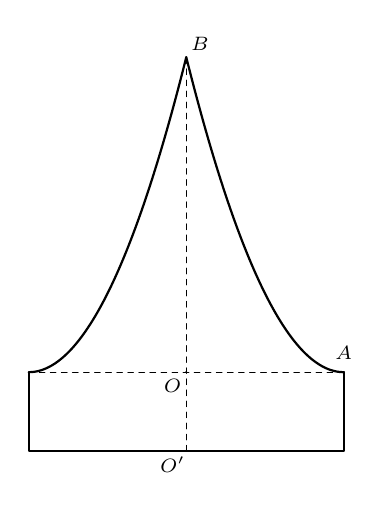
\begin{tikzpicture}[line join=round, line cap=round,>=stealth,scale=0.2]
			\path (0,0) coordinate (O)
			(10,0) coordinate (A)
			(0,20) coordinate (B)
			(0,-5) coordinate (O')
			(10,-5) coordinate (I)
			(-10,-5) coordinate (C)
			(-10,0) coordinate (D)
			;
			\draw[smooth,samples=100,thick] plot[domain=0:10](\x,{(1/5)*((\x)-10)^2})
			plot[domain=-10:0](\x,{(1/5)*((\x)+10)^2})
			;
			\draw[dash pattern=on 2pt off 2pt] (O')--(O)--(B) (A)--(D);
			\draw[thick] (A)--(I)--(C)--(D);
			\foreach \t/\g in {A/90,B/45,O/-135,O'/-135}{
				\draw[fill=black] (\t) circle (1pt) node[shift={(\g:7pt)},font=\scriptsize]{$ \t $};
			}
		\end{tikzpicture}
	}
	\loigiai{
		\immini{Ta gọi thể tích của chiếc mũ là $V$.\\
			Thể tích của khối trụ có bán kính đáy bằng $OA=10$ cm và đường cao $OO'=5$ cm là $V_1$.\\
			Thể tích của vật thể tròn xoay khi quay hình phẳng giới hạn bởi đường cong $AB$ và hai trục tọa độ quanh trục $Oy$ là $V_2$.\\
			Ta có $V=V_1+V_2$; $V_1=5\cdot 10^2\pi =500\pi $ cm$^3$.\\
			Chọn hệ trục tọa độ như hình vẽ.\\
			Do parabol có đỉnh $A$ nên nó có phương trình dạng $(P)\colon y=a(x-10)^2$.
		}
		{\begin{tikzpicture}[line join=round, line cap=round,>=stealth,font=\scriptsize,scale=0.2]
				\path (0,0) coordinate (O)
				(10,0) coordinate (A)
				(0,20) coordinate (B)
				(0,-5) coordinate (O')
				(-10,0) coordinate (C)
				;
				\draw[-stealth] (-12,0)--(0,0)--(12,0)node[below]{$x$};
				\draw[-stealth] (0,-7)--(0,22)node[left]{$y$};
				\draw[smooth,samples=100,thick] plot[domain=0:10](\x,{(1/5)*((\x)-10)^2})
				plot[domain=-10:0](\x,{(1/5)*((\x)+10)^2})
				;
				\draw[thick] (10,0) rectangle (-10,-5);
				\foreach \t/\g in {O/-135,O'/-135}{
					\draw[fill=black] (\t) circle (1pt) node[shift={(\g:7pt)},font=\scriptsize]{$ \t $};
				}
				\draw[fill=black] (A) circle (1pt)node[shift={(45:10pt)}]{$A(10;0)$};
				\draw[fill=black] (B) circle (1pt)node[right]{$B(0;20)$};
				\path (O')--(O)node[pos=0.4,left]{$5$};
				\node at ($(A)+(100:10)$) {$y=\dfrac{1}{5}(x-10)^2$};
			\end{tikzpicture}
		}\noindent
		Vì $(P)$ qua điểm $B(0;20)$ nên $a=\dfrac{1}{5}$.\\
		Do đó, $(P)\colon y=\dfrac{1}{5}(x-10)^2$. Từ đó suy ra $x=10-\sqrt{5y}$ (do $ x<10$).\\
		Suy ra $V_2=\pi \displaystyle\int\limits_0^{20}\left(10-\sqrt{5y}\right)^2\mathrm{\,d}y=\pi(3000-\dfrac{8000}{3})=\dfrac{1000}{3}\pi$ cm$^3$.\\
		Do đó $V=V_1+V_2=\dfrac{1000}{3}\pi +500\pi =\dfrac{2500}{3}\pi$ cm$^3$.
		
	}
\end{ex}
%%==========Câu 13
\begin{ex}%[2D4V3-4]
	\immini{Một chi tiết máy được thiết kế như hình vẽ bên. Các tứ giác $ABCD$, $CDPQ$ là các hình vuông cạnh $2{,}5$ (cm). Tứ giác $ABEF$ là hình chữ nhật có $BE=3{,}5$ (cm). Mặt bên $PQEF$ được mài nhẵn theo đường parabol $(P)$ có đỉnh parabol nằm trên cạnh $ EF$. Thể tích của chi tiết máy bằng
		
	}
	{\begin{tikzpicture}[scale=0.8, font=\footnotesize, line join=round, line cap=round,>=stealth,declare function={a=3;h=4.5;}]
			\path (0,0) coordinate (A)
			--++(30:a) coordinate (B)
			--++(90:a) coordinate (C)
			($(A)+(C)-(B)$) coordinate (D)
			($(A)+(180:h)$) coordinate (F)
			($(B)+(F)-(A)$) coordinate (E)
			($(D)+(180:a)$) coordinate (P)
			($(C)+(P)-(D)$) coordinate (Q)
			;
			\draw (A)--(B)--(C)--(D)--cycle (F)--(A) (D)--(P)--(Q)--(C);
			\draw[dashed] (F)--(E)--(B);
			\draw (F)..controls +(30:1) and +(-100:1)..(P)node[midway,right]{$c$};
			\draw[dashed] (E)..controls +(30:1) and +(-100:1)..(Q)node[pos=0.3,right]{$c$};
			\foreach \t/\g in {A/-90,B/-90,C/0,D/-45,E/135,F/-90,P/180,Q/135}{
				\draw[fill=black] (\t) circle (1pt) node[shift={(\g:7pt)},font=\scriptsize]{$ \t $};
			}
		\end{tikzpicture}
	}
	\choice
	{$\dfrac{395}{24}$ cm$^3$}
	{$\dfrac{50}{3}$ cm$^3$}
	{$\dfrac{125}{8}$ cm$^3$}
	{\True $\dfrac{425}{24}$ cm$^3$}
	\loigiai{
		\immini{Gọi hình chiếu của $P$, $Q$ trên $AF$ và $BE$ là $S$ và $R$.\\
			Vật thể được chia thành hình lập phương $ABCD.PQRS$ có cạnh $2{,}5$ (cm), thể tích $V_1=\dfrac{125}{8}$ cm$^3$ và phần còn lại có thể tích $V_2$.\\
			Khi đó thể tích vật thể $V=V_1+V_2=\dfrac{125}{8}+V_2$.
		}
		{\begin{tikzpicture}[scale=0.7, font=\footnotesize, line join=round, line cap=round,>=stealth,declare function={a=3;h=6;}]
				\path (0,0) coordinate (A)
				--++(30:a) coordinate (B)
				--++(90:a) coordinate (C)
				($(A)+(C)-(B)$) coordinate (D)
				($(A)+(180:h)$) coordinate (F)
				($(B)+(F)-(A)$) coordinate (E)
				($(D)+(180:a)$) coordinate (P)
				($(C)+(P)-(D)$) coordinate (Q)
				($(A)+(P)-(D)$) coordinate (S)
				($(B)+(Q)-(C)$) coordinate (R)
				($(F)!0.5!(S)$) coordinate (M)
				($(M)+(90:2)$) coordinate (M_1)
				($(E)!0.5!(R)$) coordinate (K)
				($(K)+(90:2)$) coordinate (K_1)
				;
				\path[name path=d1] (F)..controls +(30:1) and +(-100:1)..(P);
				\path[name path=d2] (E)..controls +(30:1) and +(-100:1)..(Q);
				\path[name path=d3] (M)--(M_1);
				\path[name path=d4] (K)--(K_1);
				\path[name intersections={of=d1 and d3,by=N}];
				\path[name intersections={of=d2 and d4,by=H}];
				\fill[gray!30] (N)--(M)--(K)--(H)--cycle;
				\draw (A)--(B)--(C)--(D)--cycle (F)--(A) (D)--(P)--(Q)--(C) (P)--(S) (N)--(M);
				\draw[dashed] (F)--(E)--(B) (Q)--(R)--(S) (M)--(K)--(H) (N)--(H);
				\draw (F)..controls +(30:1) and +(-100:1)..(P);
				\draw[dashed] (E)..controls +(30:1) and +(-100:1)..(Q);
				\draw[-stealth] (A)--++(0:1)node[below]{$x$};
				\draw[-stealth] (F)--++(90:1.5*a)node[left]{$y$};
				\foreach \t/\g in {A/-90,B/-90,C/0,D/-45,E/115,F/-90,P/180,Q/135,S/-90,R/-90,N/90,M/-90,K/-90,H/135}{
					\draw[fill=black] (\t) circle (1pt) node[shift={(\g:7pt)},font=\scriptsize]{$ \t $};
				}
			\end{tikzpicture}
		}\noindent
		Đặt hệ trục $Oxyz$ sao cho $O$ trùng với $F$, $Ox$ trùng với $FA$, $Oy$ trùng với tia $Fy$ song song với $AD$. Khi đó Parabol $(P)$ có phương trình dạng $y=ax^2$, đi qua điểm $P\left(1;\dfrac{5}{2}\right)$ do đó $a=\dfrac{5}{2}\Rightarrow y=\dfrac{5}{2}{x^2}$.\\
		Cắt vật thể bởi mặt phẳng vuông góc với $Ox$ và đi qua điểm $M(x;0;0)$, $0\le x\le 1$ ta được thiết diện là hình chữ nhật $MNHK$ có cạnh là $ MN=\dfrac{5}{2}x^2$ và $ MK=\dfrac{5}{2}$ do đó diện tích $S(x)=\dfrac{25}{4}x^2$.\\
		Áp dụng công thức thể tích vật thể ta có $V_2=\displaystyle\int\limits_0^1\dfrac{25}{4}x^2\mathrm{\,d}x=\dfrac{25}{12}$.\\
		Từ đó $V=\dfrac{125}{8}+\dfrac{25}{12}=\dfrac{425}{24}\approx17{,}7$ cm$^3$.
		
	}
\end{ex}

%%==========Câu 14
\begin{ex}%[2D4V3-4]
	Bổ dọc một quả dưa hấu ta được thiết diện là hình elip có trục lớn $28$ cm, trục nhỏ $25$ cm. Biết cứ $1000$ m$^3$ dưa hấu sẽ làm được cốc sinh tố giá $20000$ đồng. Hỏi từ quả dưa hấu trên có thể thu được bao nhiêu tiền từ việc bán nước sinh tố? Biết rằng bề dày vỏ dưa không đáng kể.
	\choice
	{\True $183000$ đồng} 
	{$180000$ đồng} 
	{$185000$ đồng} 
	{$190000$ đồng}
	\loigiai{ 
		Đường elip có trục lớn $28$ cm, trục nhỏ $25$ cm có phương trình
		\[\dfrac{y^2}{\left(\dfrac{25}{2}\right)^2}=1\Leftrightarrow y^2=\left(\dfrac{25}{2}\right)^2\left(1-\dfrac{x^2}{14^2}\right)\Leftrightarrow y=\pm \dfrac{25}{2}\sqrt{1-\dfrac{x^2}{14^2}}.\]
		Do đó thể tích quả dưa là
		{\allowdisplaybreaks
			\begin{eqnarray*}
				V
				&=& \pi \int\limits_{-14}^{14}\left(\dfrac{25}{2}\sqrt{1-\dfrac{x^2}{14^2}} \right)^2\mathrm{d}x\\
				&=& \pi\left(\dfrac{25}{2}\right)^2\displaystyle\int\limits_{-14}^{14}\left(1-\dfrac{x^2}{14^2}\right)^2\mathrm{d}x\\
				&=&\pi\left(\dfrac{25}{2}\right)^2 \cdot \left(x-\dfrac{x^3}{3\cdot 14^2}\right) \Big|_{-14}^{14}\\
				&=& \pi\left(\dfrac{25}{2}\right)^2 \cdot \dfrac{56}{3}\\
				&=& \dfrac{8750\pi}{3} \;\;\text{cm}^3.
			\end{eqnarray*}
		}
		Do đó tiền bán nước thu được là $\dfrac{8750\pi \cdot 20000}{3\cdot 1000}\approx 183259$ đồng.
	} 
\end{ex} 
%------------------------------------------------------------
% \begin{ex}%[2D4V3-4]%Câu 1.
% 	\immini{Có một cốc nước thủy tinh hình trụ, bán kính trong lòng đáy cốc là $6\,\text{cm}$, chiều cao lòng cốc là $10\,\text{cm}$ đang đựng một lượng nước. Tính thể tích lượng nước trong cốc, biết khi nghiêng cốc nước vừa lúc khi nước chạm miệng cốc thì đáy mực nước trùng với đường kính đáy.
% 		\choice
% 		{\True $240$\,cm$^3$}
% 		{$240\pi$ \,cm$^3$}
% 		{$120$\,cm$^3$}
% 		{$120\pi$ \,cm$^3$}}
% 	{\begin{tikzpicture}[scale=0.7, font=\footnotesize,line join=round, line cap=round, >=stealth]
% 			\begin{scope}[shift={(0,0)}]
% 				\def\a{1.5}
% 				\def\b{.5}
% 				\def\h{4}
% 				\path
% 				(0,0) coordinate (M)
% 				($(M)+(2*\a,0)$) coordinate (N)
% 				($(M)!0.5!(N)$)coordinate (O)
% 				($(M)+(0,\h)$) coordinate (M')
% 				($(N)+(0,\h)$) coordinate (N')
% 				($(O)+(0,\h)$) coordinate (O')
% 				($(M')!0.6!(M)$)coordinate (A)
% 				($(N')!0.6!(N)$)coordinate (B)
% 				;
% 				\fill[black!15] (A) arc (180:0:\a cm and \b cm)--(N)--(M) arc (-180:0:\a cm and \b cm)--(M)--(A);
% 				\draw(M)--(M') (N)--(N');
% 				\draw[dashed,thin] (M) arc (180:0:\a cm and \b cm);
% 				\draw[dashed,thin] (A) arc (180:0:\a cm and \b cm);
% 				\draw (O') ellipse (\a cm and \b cm)	(M) arc (-180:0:\a cm and \b cm) (A) arc (-180:0:\a cm and \b cm);
% 			\end{scope}
% 			\begin{scope}[rotate=-70,shift={(0,6)}]
% 				\def\a{1.5}
% 				\def\b{.5}
% 				\def\h{4}
% 				\path
% 				(0,0) coordinate (M)
% 				($(M)+(2*\a,0)$) coordinate (N)
% 				($(M)!0.5!(N)$)coordinate (O)
% 				($(M)+(0,\h)$) coordinate (M')
% 				($(N)+(0,\h)$) coordinate (N')
% 				($(O)+(0,\h)$) coordinate (O')
% 				($(M')!0.6!(M)$) coordinate (A)
% 				($(N')!0.6!(N)$) coordinate (B)
% 				;
% 				\fill[black!15]  (2.1,-.45)--(.8,.45) .. controls +(70:2) and +(180:0) ..(N') (N').. controls +(-90:.3) and +(180:0) ..(N).. controls +(-90:.3) and +(0:0.3) ..(2.1,-.45);
% 				\draw(M)--(M') (N)--(N');
% 				\draw[dashed,thin] (M) arc (180:0:\a cm and \b cm);
% 				\draw (O') ellipse (\a cm and \b cm)	(M) arc (-180:0:\a cm and \b cm);
				
% 				\draw[dashed] (2.1,-.45)--(.8,.45) .. controls +(70:2) and +(180:0) ..(N') (1.5,0)--(N');
% 				\draw (2.1,-.45) .. controls +(40:1) and +(180:0) ..(N') ;
				
% 			\end{scope}
% 	\end{tikzpicture}} 
	
% 	\loigiai{
% 		\textbf{Cách 1.} 
% 		\begin{center}
% 			\begin{tikzpicture}[scale=1, font=\footnotesize,line join=round, line cap=round, >=stealth]
% 				\path
% 				(0,0) coordinate (A)
% 				(0,3) coordinate (B)
% 				;
				
% 				\draw (A) arc (0: -90: 5 and 2) coordinate (C);
% 				\draw[dashed] (A) arc (0: 90: 4.5 and 2) coordinate (D);
% 				\coordinate (I) at ($(C)!.5!(D)$);
% 				\draw (A)--(B) (C)--(D) (I)--(B);
% 				\draw[dashed] (I)--(A);
% 				\draw 
% 				(C) .. controls +(0:0) and +(-90:1.5) ..(B).. controls +(90:1.5) and +(60:0) ..(D);
% 				\draw pic[draw, angle radius=2mm]{right angle=B--A--I};
% 				\pic[draw,"$\alpha$", angle eccentricity=0.6,angle radius=0.8cm]{angle=A--I--B};
% 				\path (A)--(I) node[above,pos=.7,sloped]{$R$};
% 				\path (C)--(I) node[above,midway,sloped]{$R$};
% 				\path (D)--(I) node[above,midway,sloped]{$R$};
% 			\end{tikzpicture}
% 		\end{center}
% 		Xét thiết diện cắt cốc thủy tinh vuông góc với đường kính tại vị trí bất kỳ có  
% 		$$S(x)=\dfrac{1}{2}\sqrt{R^2-x^2}\cdot \sqrt{R^2-x^2}\cdot \tan \alpha= \dfrac{1}{2}\left( R^2-x^2 \right)\tan \alpha.$$
% 		Thể tích hình cái nêm là: $V=\dfrac{1}{2}\tan \alpha \displaystyle\int\limits_{-R}^{R}{\left( R^2-x^2 \right)}\mathrm{\,d}x=\dfrac{2}{3}R^3\tan \alpha $.\\
% 		Thể tích khối nước tạo thành khi nguyên cốc có hình dạng cái nêm nên $V_{kn}=\dfrac{2}{3}R^3\tan \alpha $. \\
% 		$\Rightarrow V_{kn}=\dfrac{2}{3}R^3\cdot \dfrac{h}{R}=240\,cm^3$.\\
% 		\textbf{Cách 2.} 
% 		\begin{center}
% 			\begin{tikzpicture}[scale=1, font=\footnotesize,line join=round, line cap=round, >=stealth]
% 				\path
% 				(0,0) coordinate (O)
% 				(0,4) coordinate (O')
% 				(7,0) coordinate (J)
% 				(7,4) coordinate (J')
% 				(9,0) coordinate (x)
% 				($(J)!.5!(J')$) coordinate (I)
% 				($(O)!.5!(O')$) coordinate (I')
% 				;
% 				\fill[cyan!20] (J)--(O) .. controls +(82:0.6) and +(180:0.6) ..
% 				(6.15,3.15)--(7.85,.9).. controls +(180:0.05) and +(0:.6) ..
% 				(7,0);
% 				\draw[->] (O)--(x);
% 				\draw[dashed,name path=OB] 
% 				(O) .. controls +(82:0.6) and +(180:0.6) ..
% 				(6.15,3.15)coordinate (B)--(7.85,.9) coordinate (A);
% 				\draw (0,2) ellipse (1 and 2) (O)--(O') (O')--(J') ;
% 				\draw (J) arc (-90: 90: 1 and 2);
% 				\draw[dashed] (J) arc (-90: 90: -1 and 2) (J)--(J') ;
% 				\draw[dashed,name path=II'] (I)--(I');
% 				\path [name intersections={of=OB and II',by=H}];
% 				\coordinate (E) at ($(J)!(H)!(O)$);
% 				\coordinate (N) at ($(O)!.55!(A)$);
				
% 				\path (intersection of H--E and O--I) coordinate (F);
% 				\coordinate (n) at ($(F)!-3!(N)$);
% 				\path[name path=FN] (N)--(n);
% 				\path [name intersections={of=OB and FN,by=M}];
				
% 				\fill[orange!50] (M) .. controls +(-90:1) and +(180:.5) ..(E) .. controls +(0:.5) and +(180:0) ..(N);
% 				\draw[dashed] (H)--(E) (M)--(N) (H)--(N) (O)--(I);
% 				\draw[dashed] (M) .. controls +(-90:1) and +(180:.5) ..(E);
% 				\draw (E) .. controls +(0:.5) and +(180:0) ..(N) (O)--(A);
% 				\draw[<->] ($(O)+(0,-.3)$)--($(E)+(0,-.3)$) node[fill=white,midway,sloped]{$x$};
% 				\draw[<->] ($(O')+(0,.3)$)--($(J')+(0,.3)$) node[fill=white,midway,sloped]{$10$ cm};
% 				\draw[<->] ($(J)+(1.5,0)$)--($(J')+(1.5,0)$) node[fill=white,midway,sloped]{$12$ cm};
% 				\draw[->] ($(E)+(.5,.3)$)--($(E)+(.8,-.5)$) node[below] {$S(x)$};
% 				\pic[draw,"$\alpha$", angle eccentricity=1.1,angle radius=2cm]{angle=J--O--I};
% 				\node[above right] at (F) {$\beta$};
% 				\foreach \x/\g in {H/90,E/-70,F/120,N/-90,M/90,I/0,J/-90,O/-120} \fill[black] (\x) circle (1pt)+(\g:.3) node {$\x$};
% 			\end{tikzpicture}
% 		\end{center}
% 		Dựng hệ trục tọa độ $Oxyz$.\\
% 		Gọi $S\left( x \right)$ là diện tích thiết diện do mặt phẳng có phương vuông góc với trục $Ox$ với khối nước, mặt phẳng này cắt trục $Ox$ tại điểm có hoành độ $h\ge x\ge 0$.\\
% 		Gọi $\widehat{IOJ}=\alpha ,\,\widehat{FHN}=\beta ,\,OE=x$\\
% 		$\tan \alpha =\dfrac{IJ}{OJ}=\dfrac{6}{10}=\dfrac{EF}{OE}\Rightarrow EF=\dfrac{6x}{10}\Rightarrow HF=6-\dfrac{6x}{10}$.\\
% 		$\cos \beta =\dfrac{HF}{HN}=\dfrac{6-\dfrac{6x}{10}}{6}=1-\dfrac{x}{10}\Rightarrow \beta =\arccos \left( 1-\dfrac{x}{10} \right)$\\
% 		%-------------------------------------
% 		$S\left( x \right)=S_{\text{hình quạt}}-S_{HMN}=\dfrac{1}{2}HN^2\cdot 2\beta -\dfrac{1}{2}HM\cdot HN\cdot \sin 2\beta $\\
% 		%-------------------------------------
% 		$\Rightarrow S\left( x \right)=6^2\arccos \left( 1-\dfrac{x}{10} \right)-\dfrac{1}{2}\cdot 6\cdot 6\cdot 2\left( 1-\dfrac{x}{10} \right)\sqrt{1-\left( 1-\dfrac{x}{10} \right)^2}$\\
% 		$\Rightarrow V=\displaystyle\int\limits_{0}^{10}{S\left( x \right) \,\mathrm{d}x}=\displaystyle\int\limits_{0}^{10}{\left( 36\arccos \left( 1-\dfrac{x}{10} \right)-36\left( 1-\dfrac{x}{10} \right)\sqrt{1-\left( 1-\dfrac{x}{10} \right)^2} \right)\,\mathrm{d}x}=240$.}
% \end{ex}
%------------------------------------------------------------
% \begin{ex}%[2D4V3-4]%Câu 2.
% 	\immini{Cho vật thể đáy là hình tròn có bán kính bằng 1 (tham khảo hình vẽ). Khi cắt vật thể bằng mặt phẳng vuông góc với trục $Ox$ tại điểm có hoành độ $x\ \left( -1\le x\le 1 \right)$ thì được thiết diện là một tam giác đều. Thể tích $V$ của vật thể đó là
% 		\choice
% 		{$V=\sqrt{3}$}
% 		{$V=3\sqrt{3}$}
% 		{\True $V=\dfrac{4\sqrt{3}}{3}$}
% 		{$V=\pi $}}
% 	{\includegraphics[scale=0.4]{images/Cau2_C4B3CD3.png} }
% 	\loigiai{
% 		\immini{
% 			Do vật thể có đáy là đường tròn và khi cắt bởi mặt phẳng vuông góc với trục $Ox$ được thiết diện là tam giác đều do đó vật thể đối xứng qua mặt phẳng vuông góc với trục $Oy$ tại điểm $O$.\\
% 			Cạnh của tam giác đều thiết diện là  $a=2\sqrt{1-x^2}$.\\
% 			Diện tích tam giác thiết diện là  
% 			$$S=\dfrac{a^2\sqrt{3}}{4}=\left( 1-x^2 \right)\sqrt{3}.$$
% 		}
% 		{\begin{tikzpicture}[scale=0.7, font=\footnotesize,line join=round, line cap=round, >=stealth]
% 				\path
% 				(0,0) coordinate (O)
% 				(60:3) coordinate (A)
% 				(-60:3) coordinate (B)
% 				($(A)!.5!(B)$) coordinate (x)
% 				;
% 				\draw (O) circle (3) (O)--(A)--(B);
% 				\draw[->] (-4,0) -- (4,0)node[below] {$x$};
% 				\draw[->] (0,-4) -- (0,4)node[right] {$y$};
% 				\path (A)--(B) node[above right,midway]{$\sqrt{1-x^2}$};
% 				\foreach \x/\g in {O/-120,x/-70} \fill[black] (\x) circle (1pt)+(\g:.3) node {$\x$};
% 		\end{tikzpicture}}
% 		\noindent
% 		Thể tích khối cần tìm là 
% 		$$V=2\displaystyle\int\limits_{0}^{1}{Sdx}=2\displaystyle\int\limits_{0}^{1}{\sqrt{3}\left( 1-x^2 \right)=\left. 2\sqrt{3}\left( x-\dfrac{x^3}{3} \right) \right|_{0}^{1}=\dfrac{4\sqrt{3}}{3}}.$$
% 	}
% \end{ex}
% %------------------------------------------------------------
% \begin{ex}%[2D4V3-4]%Câu 3.
% 	Sân vận động Sport Hub (Singapore) là sân có mái vòm kỳ vĩ nhất thế giới. Đây là nơi diễn ra lễ khai mạc Đại hội thể thao Đông Nam Á được tổ chức tại Singapore năm $2015$. Nền sân là một elip $\left( E \right)$ có trục lớn dài $150m$, trục bé dài $90m$ (hình vẽ). Nếu cắt sân vận động theo một mặt phẳng vuông góc với trục lớn của $\left( E \right)$và cắt elip ở $M,N$ (hình vẽ) thì ta được thiết diện luôn là một phần của hình tròn có tâm $I$ (phần tô đậm trong hình 4) với $MN$ là một dây cung và góc $\widehat{MIN}=90^{\circ}.$ Để lắp máy điều hòa không khí thì các kỹ sư cần tính thể tích phần không gian bên dưới mái che và bên trên mặt sân, coi như mặt sân là một mặt phẳng và thể tích vật liệu là mái không đáng kể. Hỏi thể tích xấp xỉ bao nhiêu?
% 	\begin{center}
% 		{\includegraphics[scale=0.8]{images/Cau3_C4B3CD3.png}\\
% 			\begin{tikzpicture}[scale=1, font=\footnotesize,line join=round, line cap=round, >=stealth]
% 				\path
% 				(0,0) coordinate (O)
% 				(-2,0) coordinate (A)
% 				(2,0) coordinate (B)
% 				(70: 2 and 1) ellipse  coordinate (M)
% 				(-70: 2 and 1) ellipse  coordinate (N)
% 				;
% 				\draw (O) ellipse (2 and 1) (M)--(N) (A)--(B);
% 				\fill[black] (B) circle (1pt);
% 				\fill[black] (A) circle (1pt);
% 				\foreach \x/\g in {M/90,N/-90} \fill[black] (\x) circle (1pt)+(\g:.3) node {$\x$};
% 				\begin{scope}[shift={(5,-0)}]
% 					\path (0,0) coordinate (I) (40:2)   coordinate (M)
% 					(140:2)  coordinate (N) ;
% 					\draw (I) circle (2) (M)--(N);
					
					
% 					\clip (-2,1.28) rectangle (2,2);
% 					\fill[black!15] (I) circle (2);
% 					\draw (I) circle (2) (M)--(N);
% 				\end{scope}
% 				\foreach \x/\g in {M/45,N/135,I/-90} \fill[black] (\x) circle (1pt)+(\g:.3) node {$\x$};
% 		\end{tikzpicture} }
% 	\end{center}
% 	\choice
% 	{$57793$ m$^3$}
% 	{\True $115586$ m$^3$}
% 	{$32162$ m$^3$}
% 	{$101793$ m$^3$}
% 	\loigiai{
% 		\begin{center}
% 			\includegraphics[scale=0.8]{images/Cau3_C4B3CD3_g.png}
% 		\end{center}
% 		Chọn hệ trục như hình vẽ\\
% 		Ta cần tìm diện tích của $S\left( x \right)$thiết diện.\\
% 		Gọi $d\left( O,MN \right)=x$\\
% 		$\left( E \right)\colon\dfrac{x^2}{75^2}+\dfrac{y^2}{45^2}=1.$\\
% 		Lúc đó $MN=2y=2\sqrt{45^2\left( 1-\dfrac{x^2}{75^2} \right)}=90\sqrt{1-\dfrac{x^2}{75^2}}$\\
% 		$\Rightarrow R=\dfrac{MN}{\sqrt{2}}=\dfrac{90}{\sqrt{2}}.\sqrt{1-\dfrac{x^2}{75^2}}\Rightarrow R^2=\dfrac{90^2}{2}\cdot \left( 1-\dfrac{x^2}{75^2} \right)$.\\
% 		$S\left( x \right)=\dfrac{1}{4}\pi R^2-\dfrac{1}{2}R^2=\left( \dfrac{1}{4}\pi -\dfrac{1}{2} \right)R^2=\left( \pi -2 \right)\dfrac{2025}{2}.\left( 1-\dfrac{x^2}{75^2} \right).$\\
% 		Thể tích khoảng không cần tìm là
% 		$$V=\displaystyle\int\limits_{-75}^{75}\left( \pi -2 \right)\dfrac{2025}{2}.\left( 1-\dfrac{x^2}{75^2} \right)\approx 115586 \,\text{m}^3.$$
% 	}
% \end{ex}
%------------------------------------------------------------
% \begin{ex}%[2D4V3-4]%Câu 4.
% 	\immini{Gọi $\left( H \right)$ là phần giao của hai khối $\dfrac{1}{4}$ hình trụ có bán kính $a$, hai trục hình trụ vuông góc với nhau như hình vẽ sau. Tính thể tích của khối $\left( H \right)$.
% 		\choice
% 		{${{V}_{\left( H \right)}}=\dfrac{a^3}{2}$}
% 		{${{V}_{\left( H \right)}}=\dfrac{3a^3}{4}$}
% 		{\True $V_{\left( H \right)}=\dfrac{2a^3}{3}$}
% 		{${{V}_{\left( H \right)}}=\dfrac{\pi a^3}{4}$}}
% 	{\includegraphics[scale=0.8]{images/Cau4_C4B3CD3_De.png}}
% 	\loigiai{
% 		\begin{center}
% 			\includegraphics[scale=0.8]{images/Cau4_C4B3CD3.png}
% 		\end{center}
% 		+ Đặt hệ toạ độ $Oxyz$ như hình vẽ, xét mặt cắt song song với mp $\left( Oyz \right)$ cắt trục $Ox$ tại $x$: thiết diện mặt cắt luôn là hình vuông có cạnh $\sqrt{a^2-x^2}$ $\left( 0\le x\le a \right)$.\\
% 		+ Do đó thiết diện mặt cắt có diện tích: $S\left( x \right)=a^2-x^2$.\\
% 		+ Vậy $V_{\left( H \right)}=\displaystyle\int\limits_{0}^{a}{S\left( x \right)\,\mathrm{\,d}x} =\displaystyle\int\limits_{0}^{a}{\left( a^2-x^2 \right)\,\mathrm{d}x} =\left. \left( a^2x-\dfrac{x^3}{3} \right) \right|_{0}^{a}$\\
% 		$=\dfrac{2a^3}{3}$}
% \end{ex}
%------------------------------------------------------------
\begin{ex}%[2D4H3-5]%Câu 5.
	Một bác thợ xây bơm nước vào bể chứa nước. Gọi $h\left( t \right)$ là thể tích nước bơm được sau $t$ giây. Cho ${h}'\left( t \right)=6at^2+2bt$ và ban đầu bể không có nước. Sau 3 giây thì thể tích nước trong bể là $90m^3$, sau $6$ giây thì thể tích nước trong bể là $504m^3$. Tính thể tích nước trong bể sau khi bơm được $9$ giây.
	\choice
	{\True $1458m^3$}
	{$600m^3$}
	{$2200m^3$}
	{$4200m^3$}
	\loigiai{
		$\displaystyle\int\limits_{0}^{3}\left( 6at^2+2bt \right)\,\mathrm{d}t=90\Leftrightarrow \left.\left( 2at^3+bt^2 \right) \right|_{0}^{3}=90\Leftrightarrow 54a+9b=90$\quad (1)\\
		$\displaystyle\int\limits_{0}^{6}\left( 6at^2+2bt \right)\,\mathrm{d}t=504 \Leftrightarrow  \left. \left( 2at^3+bt^2 \right) \right|_{0}^{6}=504\Leftrightarrow 432a+36b=504$\quad (2)\\
		Từ (1), (2) $\Rightarrow  \heva{
			& a=\dfrac{2}{3} \\ 
			& b=6.}$\\
		Sau khi bơm $9$ giây thì thể tích nước trong bể là\\
		$V=\displaystyle\int\limits_{0}^{9}\left(4t^2+12t \right)\,\mathrm{d}t =  \left. \left(\dfrac{4}{3}t^3+6t^2 \right) \right|_{0}^{9}=1458\; \left(m^3 \right)$.}
\end{ex}
%------------------------------------------------------------
\begin{ex}%[2D4H3-5]%Câu 6.
	Người ta thay nước mới cho một bể bơi có dạng hình hộp chữ nhật có độ sâu là $280$cm. Giả sử $h\left( t \right)$là chiều cao (tính bằng cm) của mực nước bơm được tại thời điểm $t$ giây, biết rằng tốc độ tăng của chiều cao mực nước tại giây thứ $t$ là ${h}'(t)=\dfrac{1}{500}\sqrt[3]{t}$ và lúc đầu hồ bơi không có nước. Hỏi sau bao lâu thì bơm được số nước bằng $\dfrac{3}{4}$độ sâu của hồ bơi (làm tròn đến giây)?
	\choice
	{$2$ giờ $36$ giây}
	{$2$ giờ $48$ giây}
	{\True $2$ giờ $38$ giây}
	{$2$ giờ $46$ giây}
	\loigiai{
		Gọi $x$ là thời điểm bơm được số nước bằng $\dfrac{3}{4}$ độ sâu của bể ($x$ tính bằng giây).
		Ta có
		\begin{eqnarray*}
			&&\displaystyle\int\limits_0^x{\dfrac{1}{500}\sqrt[3]{t}\mathrm{\,d}t}=\dfrac{3}{4}\cdot 280\left. \Rightarrow \dfrac{3}{4}t^{\dfrac{4}{3}} \right|_0^x=105000\\
			&\Rightarrow& x\sqrt[3]{x}=140000\Rightarrow \sqrt[3]{x^4}=140000\\
			&\Rightarrow& x=\sqrt[4]{140000^3}\Rightarrow x\approx 7237{,}6242.
		\end{eqnarray*}
		Suy ra $x= 2$ giờ $38$ giây.}
\end{ex}
%------------------------------------------------------------
\Closesolutionfile{ans}
\indapan{6}{ans/ans-2-C4B3CD3_1-2-lc}

